\chapter{Hintergrund}

Um spätere Missverständnisse zu vermeiden, erklären diese Grundlagen das Basis-Verständnis einer Auswahlkomponente und grundlegendes zum Thema Browser.
Im Zusammenhang mit der Auswahlkomponente muss klar sein, welche Zustände existieren.
Um eine Basis für das Erstellen einer konsistenten Auswahlkomponente zu ermöglichen, zeigt der Browser-Abschnitt den Grund für die vorhandenen Unterschiede.
Zudem klärt eines dieser Unterkapitel den Ablauf des Rendern einer HTML-Seite und bietet ein besseres Verständnis für die Entwicklung der neuen Komponente.


\section{Ausgangslage}

Kolibri, ein von der FHNW betriebenes Toolkit, wird laufend weiterentwickelt.
Die Open Source Werkzeuge können von Entwicklern ganz einfach importiert und verwendet werden.
Um Kolibri schlank zu halten, kommen keine externen Abhängigkeiten zur Verwendung.
Mit einer VanillaJS Codebasis bietet das Tool eine breite Auswahl an, deckt aber noch nicht alle Interaktionen ab.

In diesem Projekt dient der in der Vorarbeit erstellte Fork als Ausgangslage.
Ein Merge des Branches \emph{experimental} dieses Forks und des \emph{Kolibri-16} der originalen Codebasis stellt die Aktualität sicher.
Das \texttt{SimpleInput} ist eines der Tools, welches sich bei der Implementation der neuen Auswahlkomponente als hilfreich erweisen kann.

Der Zugriff auf das Designtool Figma ermöglicht das Verwenden des existierenden Designsystems und der bereits eingebundenen Elemente. 
Der Aufbau der Elemente als Komponenten vereinfacht die Wiederverwendung. 
Der Satz von Icons kann bei Bedarf erweitert werden.

Eine weitere, wichtige Ausgangslage ist ein gemeinsames Verständnis von verwendeten Begriffen. 
Um dies sicherzustellen, beschreibt das nächste Kapitel die Zustände einer Auswahlkomponente als auch derer Elemente.
Diese Definitionen gelten im gesamten Bericht.


\section{Zustände in einer Auswahlkomponente}

Dieser Abschnitt erklärt die Zustände, welche in einer Auswahlkomponente auftreten können.
Als Ausgangslage dient eine Eingabemöglichkeit, die eine Master-Detail-Ansicht\footnotemark aufweist.
\footnotetext{
    Master beschreibt den Bereich, welcher alle möglichen Auswahlwerte enthält.  
    Detail beschreibt den Bereich, welcher den aktuell ausgewählten (selektierten) Wert enthält.
}
Zudem sind keine speziellen Voreinstellungen getroffen.
\\
Je nach Darstellung der Komponente kann diese $offen$ oder $geschlossen$ sein.
Wenn nur einer der beiden Zustände möglich ist, ist es meistens der Offene.
Im geschlossenen Status zeigt das Erscheinungsbild nur die Detail-Ansicht an, welcher mindestens den selektierten Wert anzeigt.
Eine offene Auswahlmöglichkeit stellt beide Elemente der Master-Detail-View dar.
Die Master-Ansicht zeigt alle Values einer Liste an.

Bei dem $normalen$ bzw. nicht fokussierten Status ist die Komponente nicht an- oder ausgewählt.
Wenn eine Webseite diese Komponente enthält, ist dies die standardmässige Darstellung.
Das neue Element zeigt keine Reaktion auf Interaktionen, welche in diesem Zustand geschehen. 
Als einzige Ausnahme gilt Tab, welche den Fokus auf die Komponente legen kann. 
In den meisten Erscheinungen ist nur die Detail-Ansicht sichtbar und der Master-Container ist ausgeblendet.
Wählt der Nutzer die Komponente mit der Maus oder der Tastatur an, steht sie im $Fokus$ bzw. ist sie $fokussiert$.
Bedienungen über das Keyboard beziehen sich hierbei auf den Baustein.
In den meisten Fällen ändert sich die Darstellung des Eingabefeldes z.B. durch einen blauen Rahmen.

Ist ein Wert in der Master-Ansicht ausgewählt und wird in der Detail-View angezeigt, ist dieser $selektiert$.
Die $Selektion$ wird beim Versenden eines verlinkten Formulars als Value mitgeschickt.
Sollte es eine $Selektion$ in einer Kategorie-Spalte geben, wird diese nicht mitgeschickt.
Stattdessen filtert die Kategorie-Selektion die Wert-Spalte.
Um die Auswahl anzuzeigen, ist dieser in der Liste aller Werte hervorgehoben.
In gewissen Situationen existiert noch der Zustand, dass in der Master-View ein Wert im $Highlight$ steht. 
Bestätigt der Nutzer das $Highlight$ mit der Maus, wechselt der Status auf selektiert.
Durch Hovern kann der Highlight-Wert geändert werden. 
Geschieht die Navigation durch die Werte mit der Tastatur, erhält genau ein Wert die $Cursor Position$. 
Durch das Betätigen gewisser vordefinierter Tasten ändert sich die $Cursor Position$.
Bei einer Bestätigung mit der Tastatur ändert sich der Wert der $Cursor Position$ auf selektiert.
Die letzten zwei Zustandswerte haben keinen Einfluss auf das versendete Formular und sind nur im Master zu finden.
Nachfolgend werden noch die Details zum Thema Browser geklärt.

\section{Browser \& HTML Renderer}


Die wichtigsten Aspekte von der Theorie über die populären Browser bis hin zum Ablauf des Renderings sind hier aufgeführt.
Dabei sind nur die bekanntesten Implementationen von Belang.

Ein Webbrowser dient hauptsächlich als Zugang ins Internet und zur Anzeige von Webressourcen wie HTML, CSS und JavaScript.
Er besteht aus einer Benutzeroberfläche, einer Browser- und einer Layout/Rendering-Engine.
Um diese Inhalte verständlich auf dem UI darzustellen, verwendet die Browser-Engine einen sogenannten Renderer - mehr dazu später.
Die Benutzeroberfläche dient als Schnittstelle zwischen dem Benutzer und der Datenschicht. 
Die Rendering-Engine interpretiert die gegebenen Inhalte, wobei der Renderer anhand des Inhaltstyps gewählt wird. 
Einer der Engines ist der HTML-Renderer, eine Software, welche den strukturierten Text aus dem HTML-File formatiert und mit dem gegebenen Style anzeigt.
Beim UI und der Bedienung zeigen sich die Uneinigkeiten zwischen den Browser-Herstellern, indem die Rendering-Engine den Code nicht gleich interpretiert.
Nachfolgend sind Informationen über den detaillierten Ablauf zur Anzeige eines HTML-Dokuments und die Rolle des Rendering dokumentiert.


\subsection{Ablauf Parsing \& Rendering}

Der Aufruf einer Webseite beginnt mit dem HTTP-Request auf welchen eine HTTP-Response folgt.
In diesem Bericht sind die gerade genannten Teile vor dem eigentlichen erhalten der Daten nicht weiter wichtig.
Der Response liefert schlussendlich die anzuzeigenden Daten, welche in diesem Fall die tragende Rolle spielen.

\begin{figure}[!htb]
    \centering
    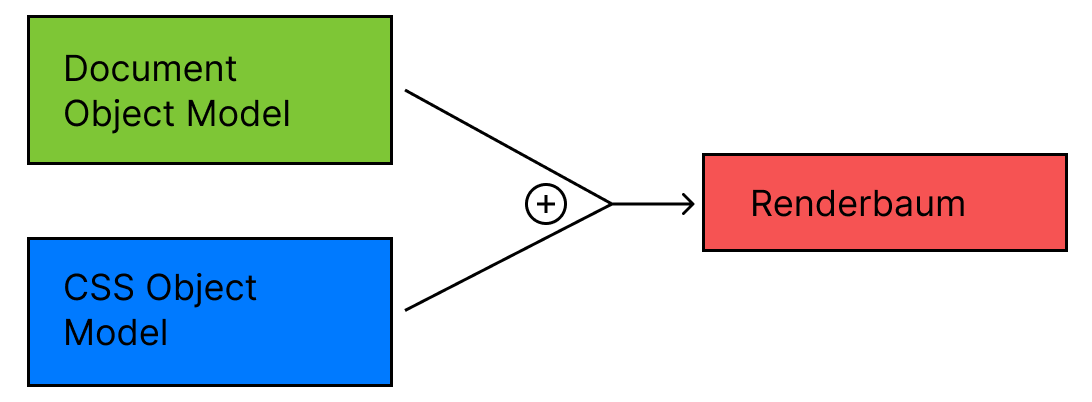
\includegraphics[width=120mm]{rendering-process.png}
    \caption{Rendering Prozess}
    \label{img:RenderingProcess}
\end{figure}

Der Entwickler schreibt Zeichen in eine HTML-Datei (Abbildung \ref{img:RenderingProcess} links oben).
Der Parser verarbeitet die einzelnen Charakter weiter zu sogenannten Tokens.
Hierbei kommt ein Satz von Regeln zur Anwendung, welche bei HTML als Tags in den Diamant-Klammern $<>$ stehen.
Durch die Definition der Struktur über die Tokens versteht der Browser den Inhalt der Dateien.
Die fertigen Tokens werden in Nodes umgewandelt, welche jeweils eigene Eigenschaften besitzen können.
Aus den entstandenen Nodes entsteht durch Verknüpfungen eine Baumstruktur - der DOM aus Abbildung \ref{img:RenderingProcess}.
Das Document Object Model (DOM) beschreibt die Eltern-Kind- und Geschwister-Beziehung der Nodes.

Wenn im HTML eine CSS-Datei (Abbildung \ref{img:RenderingProcess} links unten) verlinkt ist, muss dieses zuerst nachgefordert werden.
Nach Erhalt der Rohdaten der Style-Dateien parst der Browser diese zuerst in Charaktere und anschliessend in Tokens.
Die Baumstruktur besteht auch hier aus den Tokens gebildeten Nodes. 
Dieses Ergebnis nennt sich CSS Object Model (Abbildung \ref{img:RenderingProcess}) - kurz CSSOM - und enthält die Design-Informationen der Elemente.

Der DOM und der CSSOM sind unabhängig und der Browser kombiniert diese zu einem Renderbaum (Abbildung \ref{img:RenderingProcess} mittig).
Der resultierende Baum repräsentiert nur sichtbare Elemente, wohingegen der DOM alle Elemente enthält.
Das Layout wird im Renderbaum ergänzt und berechnet die Position und Grösse der Elemente.

Der DOM als auch der CSSOM werden parallel zum jeweiligen Parsen gerendert.
Das Rendering ist jeweils nur ein Schritt hinter dem Parser und verarbeitet dessen Resultate direkt weiter.
Dabei wird der Platz im Dokument dem Element und dem Inhalt zugewiesen und beide jeweils dort angezeigt. % todo rewrite
Extern nachgeladene Ressourcen wie Bilder können etwas länger dauern, weswegen die Seiten manchmal ohne diese vorgeladen werden.

Stösst der HTML-Parser auf ein $script$-Tag, stoppt dieser den Prozess des HTML-Parsen bis das Script fertig ausgeführt ist - ausser das Tag enthält das $async$-Attribut.
Dies dient der Sicherheit, weil JavaScript den DOM als auch CSSOM ändern kann und der Browser nicht weiss, was passieren wird.
Deswegen spielt es eine Rolle, zu welchem Zeitpunkt das Script eingebunden ist - egal ob intern oder extern. 
Während der Ausführung des Scripts führt der Browser den Prozess des CSSOM weiter fort.

Zusammengefasst kann gesagt werden, dass das Parsen von HTML-Files ein Schritt vor dem Rendern ist und dasselbe gilt für CSS-Dateien. 
Beim Script ist gut überlegt zu handeln, da der Zeitpunkt der Ausführung eine wichtige Rolle spielt.
Die verbreitetsten Browser der jeweilig aktuellsten Version mit dessen Rendering-Engines sind nachfolgend aufgeführt.


\subsection{Bekannte Implementationen}

(\cite{blinkRenderer}) Am populärsten mit ungefähr 65\% Marktanteil sind Browser auf der Chromium-Basis, welche mit dem HTML-Renderer Blink arbeiten. 
(\cite{chromiumBrowser}) Zu diesen Browser zählen Google Chrome, Brave, Microsoft Edge, Opera, Vivaldi, Samsung Internet und weitere.
(\cite{blinkRenderer}) Blink ist eine Abspaltung der Rendering-Engine WebKit und wird von der Open Source Community Chromium, Google, Intel und Samsung entwickelt.

(\cite{webkitRenderer}) WebKit selbst findet sich weiterhin im OSX Webbrowser Safari wieder, welcher mit etwa 15\% Anteil vertreten ist.
Der Renderer ist ein Fork von der KHTML-Engine und kommt von den Entwicklern Apple, Google, KDE, Nokia und weitere. 
KHTML wird nicht mehr fortgeführt.

(\cite{geckoRenderer}) Die restlichen Browser sind jeweils mit 7\% oder weniger vertreten.
(\cite{mozillaBrowser}) Dazu zählen mozilla-basierte Browser wie Firefox, Tor oder Pale Moon, welcher das HTML mit Gecko oder einem Fork dessen renderen.
(\cite{geckoRenderer}) Mozilla Foundation ist zuständig für die Weiterentwicklung dieser Rendering-Engine.
(\cite{otherRenderer}) Weiter existiert der Internet Explorer, welcher mit Trident auf Windows und mit Tasman auf Mac rendern.
Dieser Browser erhält keinen Support mehr und der Marktanteil sinkt immer weiter.
Die Renderer als auch Forks werden nur noch Maintained, aber nicht mehr weiterentwickelt.

Diese Informationen führen zur Entscheidung, dass die Implementationen der Komponente hauptsächlich auf Chrome, Safari und Firefox getestet werden.
Die Auswahl der drei Browser decken den grössten Teil der auf dem Markt verwendeten Browser und Rendering-Engines ab.
Dadurch kann eine browserübergreifende Konsistenz garantiert werden.
